\chapter{基于 CAD 模型的目标位姿追踪方法}
\label{cha:model_based_tracking}
\section{引言}
\label{sec:chapter3_intro}
目标位姿追踪技术是指通过图像信息,解算物体坐标系相对于相机坐标系的旋转矩阵以及平移向量。该技术是工业零部件抓取、增强现实等应用的基础,稳定、准确、快速的位姿追踪一直是工业视觉领域的研究重点。现有算法多使用特征点或者深度信息匹配的方法实现位姿估计与追踪,但工业现场的金属或塑料等
贫纹理零部件难以从表面提取到足够数量的特征点,导致该类算法追踪效果较差。使用机器学习方法的目标检测与姿态估计算法近年来研究火热,但预测的位姿误差较大并且算法复杂度较高,无法满足高精度追踪的要求。
区别于上述方法,基于图像边缘或轮廓的匹配方法在~1995~被提出,该方法通过寻找模型边缘与图像边缘的最优匹配以解算目标相对于相机的位姿。该类算法为基于物体三维模型的追踪方法,相比特征点方法适用范围广,对贫纹理物体仍能实现高精度追踪,并且算法复杂度较低。
但现有算法对复杂背景以及遮挡情况的鲁棒性差,易出现边缘的误匹配,导致追踪失败。

针对上述问题,本章将研究基于方向倒角匹配的模型追踪算法,构建模型边缘于场景边缘匹配的目标函数,并采用解析寻优方法实现准确的位姿寻优,使追踪精度及鲁棒性得以提升;针对遮挡问题,提出自适应权重优化算法,
通过改变模型光栅点的优化权重,降低被遮挡部分对整体寻优的影响,提高算法在目标物体被部分遮挡时的追踪精度以及鲁棒性。
本章所提追踪算法的流程如图~\ref{fig:track-flow-figure}~所示,主要分为目标函数构建以及解析寻优两部分。
\begin{figure}[b]
    \centering
  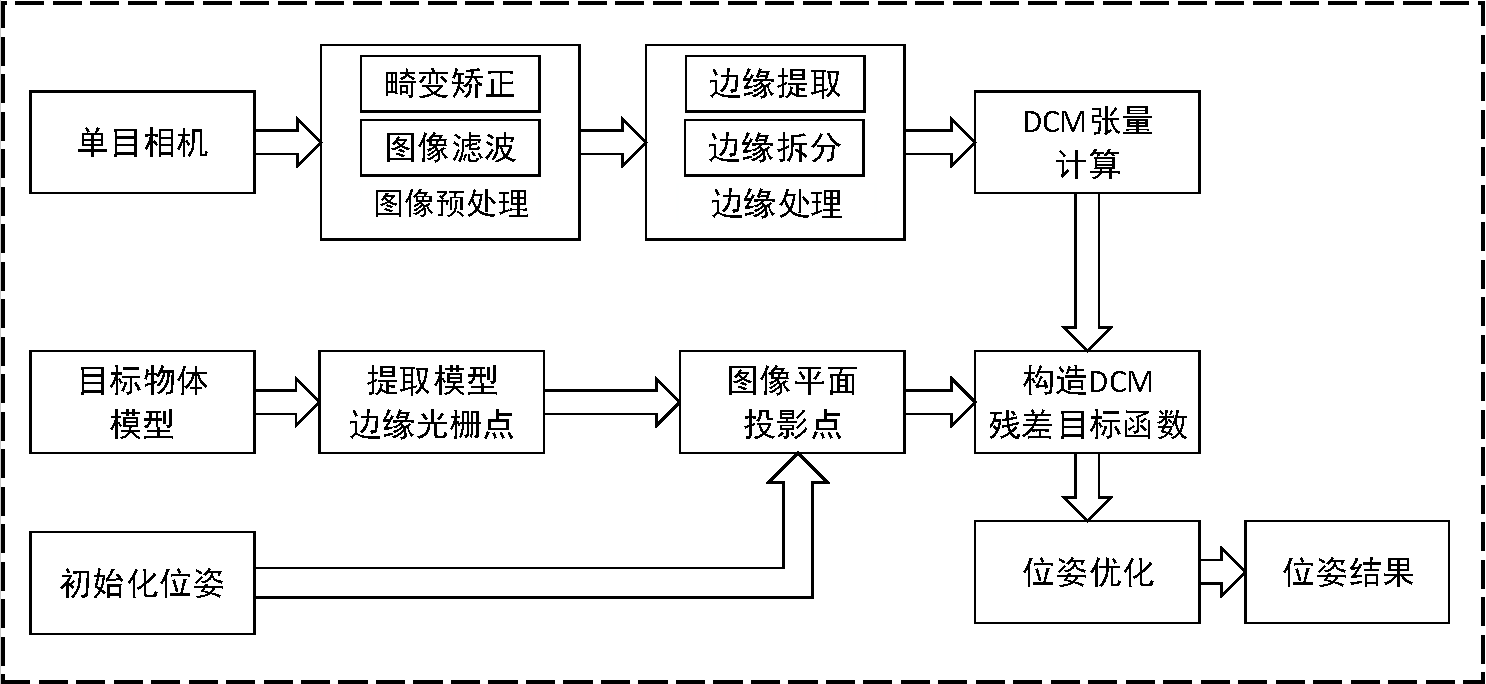
\includegraphics[height=6cm]{track-flow-figure}
    \caption{追踪算法流程图}
    \label{fig:track-flow-figure}
  \end{figure}

\section{追踪系统目标函数的建立}
\label{sec:Objective function}
系统通过寻找目标物体三维模型与场景边缘图像的最优匹配以实现位姿追踪。首先通过场景边缘图,计算方向倒角匹配(Directional Chamfer Matching,简称~DCM)张量,该张量用以代表图像坐标中各点与边缘的对应关系;之后通过初始位姿以及相机投影模型,
将目标物体三维模型投影至图像平面;最后根据投影点的模型边缘方向以及方向倒角匹配张量构建优化的目标函数。
\subsection{方向倒角匹配张量}
\label{sec:Tensor calculation}
为实现图像坐标中任一点集与场景边缘图像的匹配,常用的方法是倒角匹配(Chamfer Matching,简称~CM),该方法在图像平面寻找与目标点集的欧式距离最近的点集,作为匹配点集,以实现点集配准。
假设$M=\{m_i\}$,代表图像平面中一组待匹配的点集,其中$i=1,2,\dotsc ,|M|$;$N=\{n_j\}$,代表场景边缘图像中的边缘点集,其中$j=1,2,\dotsc ,|N|$。由此可得待匹配点集的倒角匹配误差函数如式~(\ref{equ:chap3:cm})所示,
\begin{equation}
  \label{equ:chap3:cm}
  d_{CM}(M,N)=\frac{1}{w}\sum_{m_i\in M}\min_{n_j\in N}\lVert {m_i-n_j}\rVert
\end{equation}
其中$w$代表待匹配点集的数量,$w=\lvert M\rvert$。倒角匹配方法能够将图像坐标中一点匹配至距离其图像距离最近的边缘点,该方法在待匹配点集与边缘点集图像距离较近时能够完成匹配,但其误差较大,稳定性较低,
并且当场景背景较为复杂时难以实现精确匹配。为提高边缘图像匹配精度,Tuzel等人\cite{LiuFastDirectionalChamfer2010}基于倒角匹配方案提出了方向倒角匹配方法。在原有图像距离基础上,增加方向匹配信息,使匹配过程不仅考虑二维图像距离,并且增加
方向误差。两者差异如图~\ref{fig:cm_dcm}~所示。DCM增加了方向匹配误差,结合图像距离与角度距离寻找最小配准误差,假设$\phi(\cdot)$代表二维图像中的方向运算符,即$\phi(m_i)$代表待匹配点$m_i$在图像平面中的
切向方向,$\phi(n_j)$代表场景边缘图像点~$n_j$~的边缘切向方向,构造方向倒角距离匹配误差函数如式~(\ref{equ:chap3:dcm}),其中$\lambda$代表方向误差权值,用以转换角度量纲以便与距离误差进行相加,并确定方向误差在总误差中的权重。
\begin{figure}[t] %[h]
  \centering%
  \subcaptionbox{CM 匹配\label{fig:CM}}{%    
    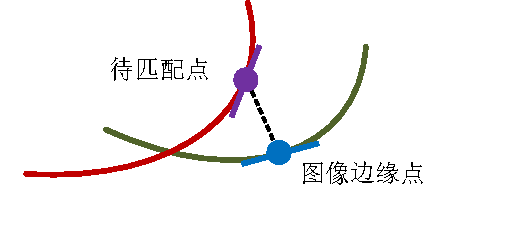
\includegraphics[height=3.2cm]{OCM}} %\hspace{1em}
  \subcaptionbox{DCM 匹配\label{fig:DCM}}{%  
    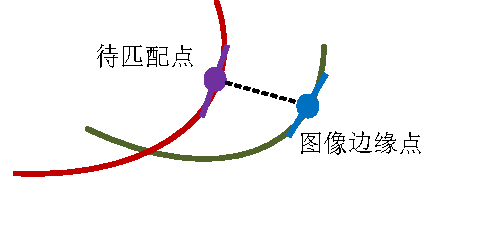
\includegraphics[height=3.2cm]{DCM}
    }
  \caption{CM-DCM 匹配对比图}
  \label{fig:cm_dcm}
\end{figure}
\begin{equation}
  \label{equ:chap3:dcm}
  d_{CM}(M,N)=\frac{1}{w}\sum_{m_i\in M}\min_{n_j\in N}(\lVert {m_i-n_j}\rVert+\lambda \lVert{\phi(m_i)-\phi(n_j)}\rVert)
\end{equation}

~DCM~边缘匹配算法将待匹配点集的方向信息加入到匹配误差函数中,降低了距离待匹配点较近的背景边缘点对配准过程的影响,大大提高匹配的精度以及鲁棒性,
本文将使用该方法构建匹配的目标函数,以计算三维模型的图像映射点集与场景边缘图像的匹配关系,最后通过优化该目标函数以得到物体相对于相机坐标系的精确位姿。

\subsection{场景~DCM~张量计算}
\label{sec:Edge Point Mapping}
场景~DCM~张量将会用于构建模型边缘与场景图像边缘的匹配目标函数,因此该张量的计算将影响模型配准以及位姿追踪的精度。为提高场景边缘图像的准确度及精度,需对输入的灰度图像进行畸变矫正以及边缘提取。
首先对实验所用的相机进行内参标定,以消除透视失真引起的畸变,提高相机投影计算的精度。对相机的标定将很大程度影响位姿追踪的精度,常用的有张正友棋盘格标定方法,本文使用~Matlab~相机标定软件包对所用相机进行标定,该软件包内置了张正友棋盘格标定方法,能够对单目、双目相机进行标定。
输入相机拍摄的图片并进行棋盘格角点识别,如图~\ref{fig:chap03:qipan}~所示,之后通过棋盘格角点的图像位置,根据~PnP~算法以得到棋盘在相机坐标系中的位姿,如图~\ref{fig:chap03:qipan_pose},最后通过最小化反投影误差的方法以计算相机内参,具体原理不再赘述。
\begin{figure}[t] %[h]
  \centering%
  \subcaptionbox{棋盘格角点识别\label{fig:chap03:qipan}}{%    
    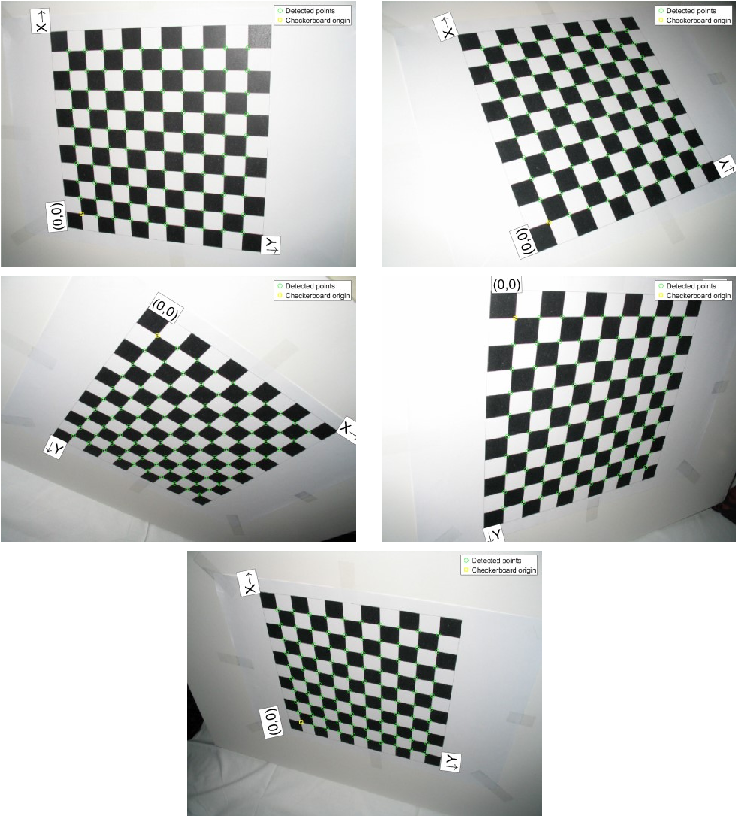
\includegraphics[height=5cm]{calib_qi_pan}} %\hspace{1em}
  \subcaptionbox{棋盘位姿\label{fig:chap03:qipan_pose}}{%  
    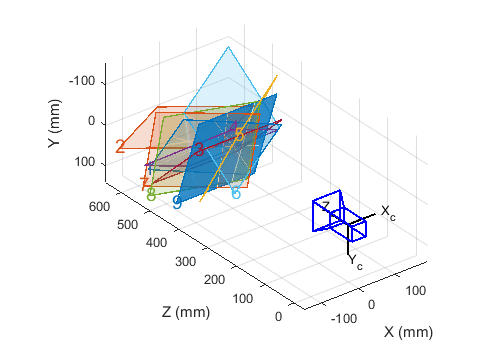
\includegraphics[height=5cm]{qipan_pose}
    }
  \caption{Matlab~相机标定图}
  \label{fig:chap03:matlab_calib}
\end{figure}
其次对灰度图像进行边缘提取,本文对比了~Canny~边缘提取算子以及
~LSD~边缘提取算法,这两种方法都是基于图像的梯度计算。像素点的梯度代表该点在图像横、纵坐标轴~$i,j$~上的灰度值变化,它是一个既有大小也有方向的矢量。记~$z=f(x,y)$~代表
图像坐标中像素点~$(x,y)$~的灰度值,由此可得该点梯度为:
\begin{equation}
grad(x,y)=\frac{\partial f}{\partial x}\vec i+\frac{\partial f}{\partial y}\vec j
\end{equation}
假设~$G_i$~和~$G_j$~分别代表~$i$~方向和~$j$~方向的梯度,则该点梯度表示为:
\begin{equation}
  \nabla f(x,y)=[G_i,G_j]^T=\left[\frac{\partial f}{\partial x},\frac{\partial f}{\partial y}\right]^T
\end{equation}
由此可得该像素点的梯度幅值与方向为:
\begin{equation}
  \left\{
    \begin{aligned}{}
    mag(\nabla f)&=g(x,y)=\sqrt{\frac{\partial ^2f}{\partial x^2}+\frac{\partial ^2f}{\partial y^2}} \\
    \phi(x,y)&=\arctan\left(\left| \frac{\partial f}{\partial y} \middle / \frac{\partial f}{\partial x}\right|\right)
    \end{aligned}
    \right.
\end{equation}
由于图像像素点为离散坐标点集,因此图像灰度值函数也为离散函数。计算方向梯度的方法有很多,最简单的梯度近似计算方法如式~(\ref{equ:chap3:tidu_jisuan}),但由于单像素点计算梯度易受噪音以及误差
影响,因此出现了很多改进方法。
\begin{equation}
  \label{equ:chap3:tidu_jisuan}
  \left\{
    \begin{aligned}{}
    G_i&=f(x,y)-f(x-1,y) \\
    G_j&=f(x,y)-f(x,y-1)
    \end{aligned}
    \right.
\end{equation}

Canny~算子是一种改进的梯度计算方法,其使用卷积算子来计算像素点梯度。该方法在保证计算速度的前提下提高了梯度计算的准确度,通过灰度图像与特定矩阵,如式~(\ref{equ:chap3:juanji})~所示,的卷积以得到梯度的大小和方向。
\begin{equation}
  \label{equ:chap3:juanji}
s_i=\left[\begin{matrix}
  -1 & 1\\
  -1 & 1\\
\end{matrix}\right],
s_j=\left[\begin{matrix}
  1 & 1\\ 
  -1 & -1
\end{matrix}\right]
\end{equation}

该算子是一种多级边缘检测算法,其目标是实现最优的边缘检测,最优边缘检测的含义是\footnote{节选自:https://en.wikipedia.org/wiki/Canny\_edge\_detector}:
\begin{itemize}
  \item 好的检测:算法能够尽可能多地标识出图像中的实际边缘
  \item 好的定位:标识出的边缘要与实际图像中的实际边缘尽可能接近
  \item 最小响应:边缘只能标识一次,并且可能存在的图像噪音不应标识为边缘
\end{itemize}

Canny~边缘提取算法首先通过卷积矩阵计算灰度图像上各像素点的梯度大小以及方向,之后使用梯度幅值的高低双阈值滤波对像素点进行筛选,经过高阈值过滤后的图像为强边缘,低阈值过滤后的图像为弱边缘,在强边缘基础上增加
距离较近的弱边缘,作为最后的边缘提取结果。高阈值过滤能够将噪音造成的边缘去除,而低阈值过滤得到的结果是对强边缘的补充,由于场景存在一些梯度较低的不明显边缘,强阈值过滤将会错误地将其去除,而
这类弱边缘常会与强边缘相连接,因此需要使用弱边缘对强边缘进行补足,以得到完整的边缘提取结果。

LSD~边缘提取算法是一种直线段检测算法,该算法对直边缘的提取能够得到连续的直线,对周围噪声的抑制效果良好,但对于曲边缘的提取是通过直线段拟合完成的,因此对于曲向边缘以及弱边缘的提取效果较差。
LSD~区别于普通边缘检测算法,其目的是寻找梯度变化明显的直线边缘。该算法通过各像素点的梯度方向进行分类,当某些像素点的图像位置相邻且方向相近时,就能构成直线段。
因此该方法的核心是寻找梯度方向相近的邻近像素点集,使其构成直线段候选区域,并对所得到的预选直线段区域进行合并和判断,最后得到场景直线段结果。

如图~\ref{fig:chap03:edge_extra}~所示为边缘提取算法对比图。其中图~\ref{fig:chap03:edge_yuanshi}~为输入的原始图像,图~\ref{fig:chap03:canny}~为使用~Canny~算子提取的边缘结果,图
~\ref{fig:chap03:lsd}~为~LSD~边缘提取结果。对比可知,Canny~算子提取结果含有非常丰富的细节信息,并且其边缘由边缘点构成,多为间断的分隔点;而~LSD~算法提取的边缘细节信息较为简洁,仅对
效果明显的直线边缘进行提取,有效抑制了噪音的影响,但对细节的提取不够强,容易遗失物体的某些弱边缘。本文通过对比发现,Canny~算子较为适用于背景简单的情况,在该类环境中为了保证有效地提取目标
物体表面的全部边缘,需要保留更多的边缘细节,因此使用~Canny~算子能够获得精度更高的边缘提取结果;而~LSD~算法适用于背景复杂的情况,由于复杂背景会存在较多噪音,需要过滤细小背景边缘的影响,增强目标物体表面强边缘的提取效果,以使追踪算法对复杂背景的
鲁棒性增强。

\begin{figure}[t] %[h]
  \centering%
  \subcaptionbox{原始图片\label{fig:chap03:edge_yuanshi}}{%    
    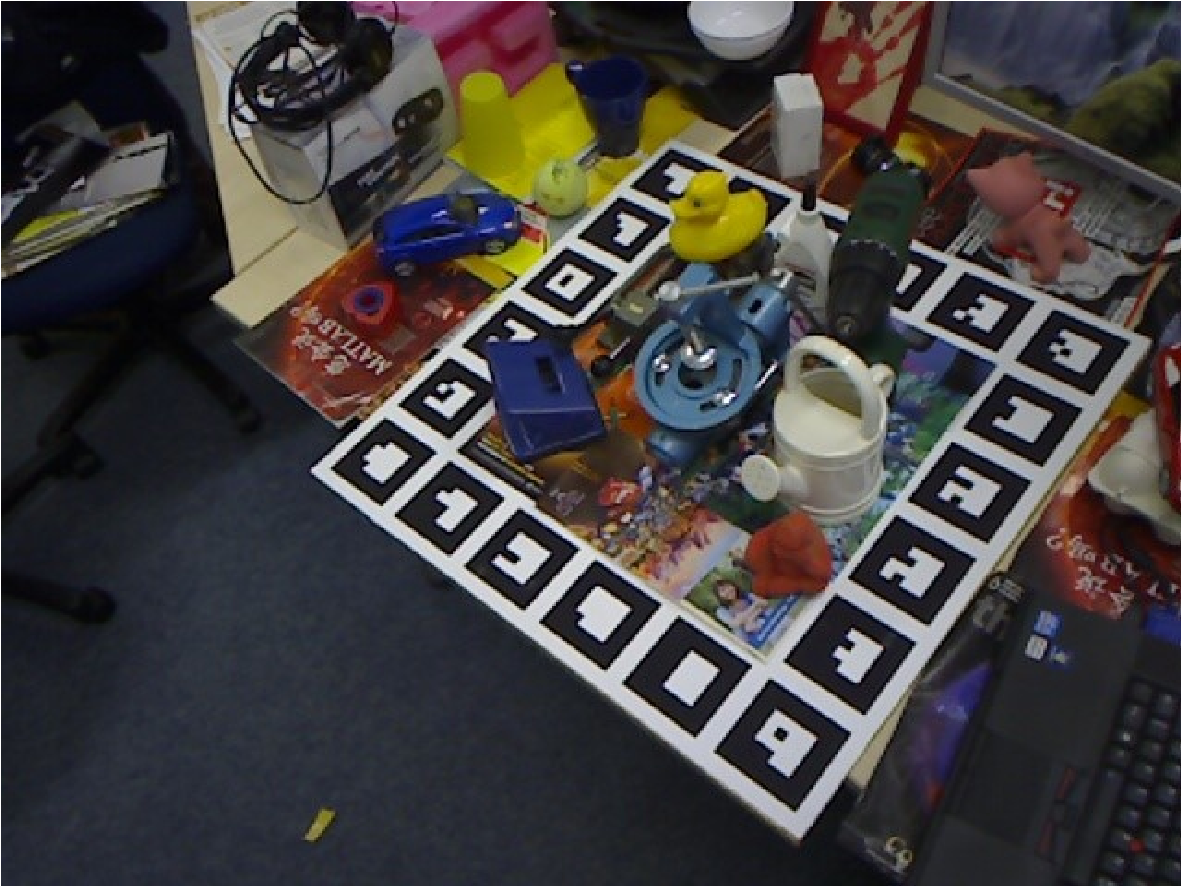
\includegraphics[height=3.5cm]{edge_yuanshi}} %\hspace{1em}
  \subcaptionbox{Canny~算子提取\label{fig:chap03:canny}}{%  
    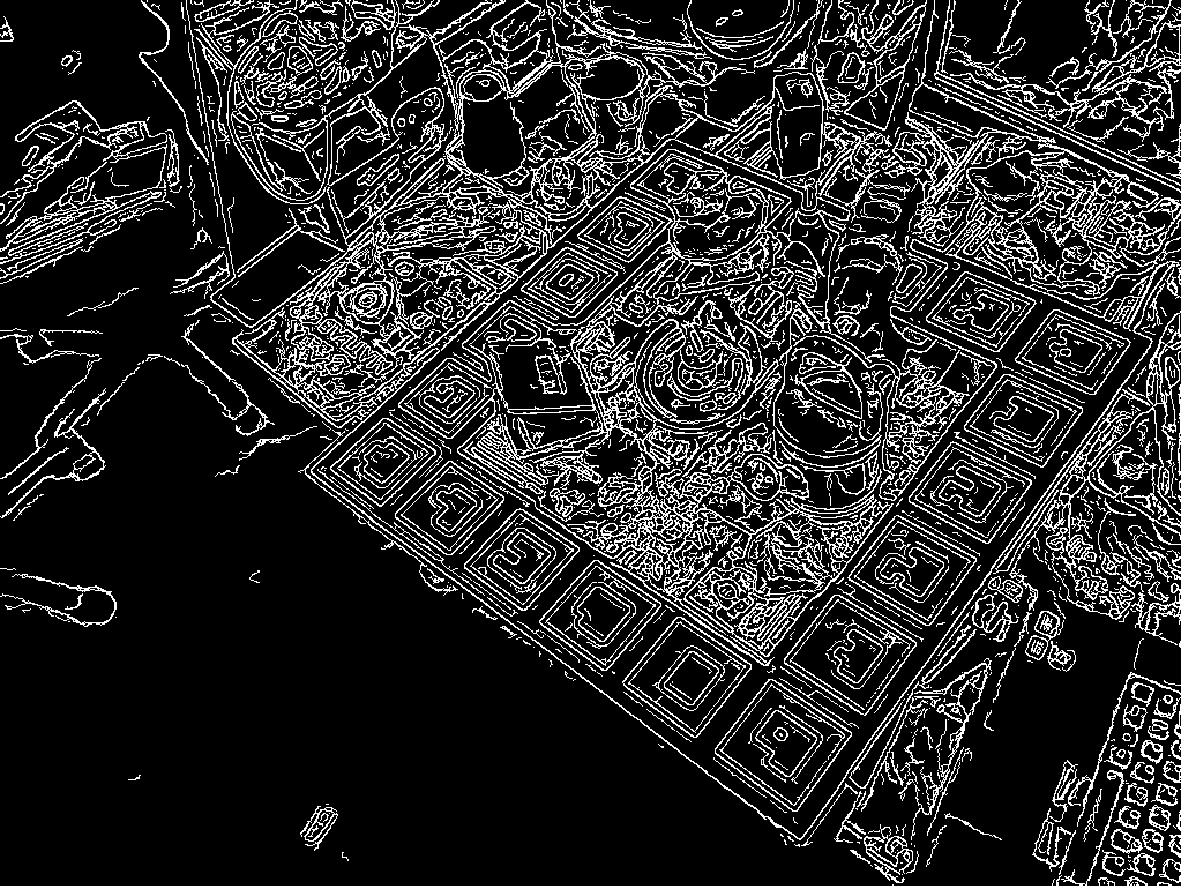
\includegraphics[height=3.5cm]{canny}
  }
  \subcaptionbox{LSD~边缘提取\label{fig:chap03:lsd}}{%  
    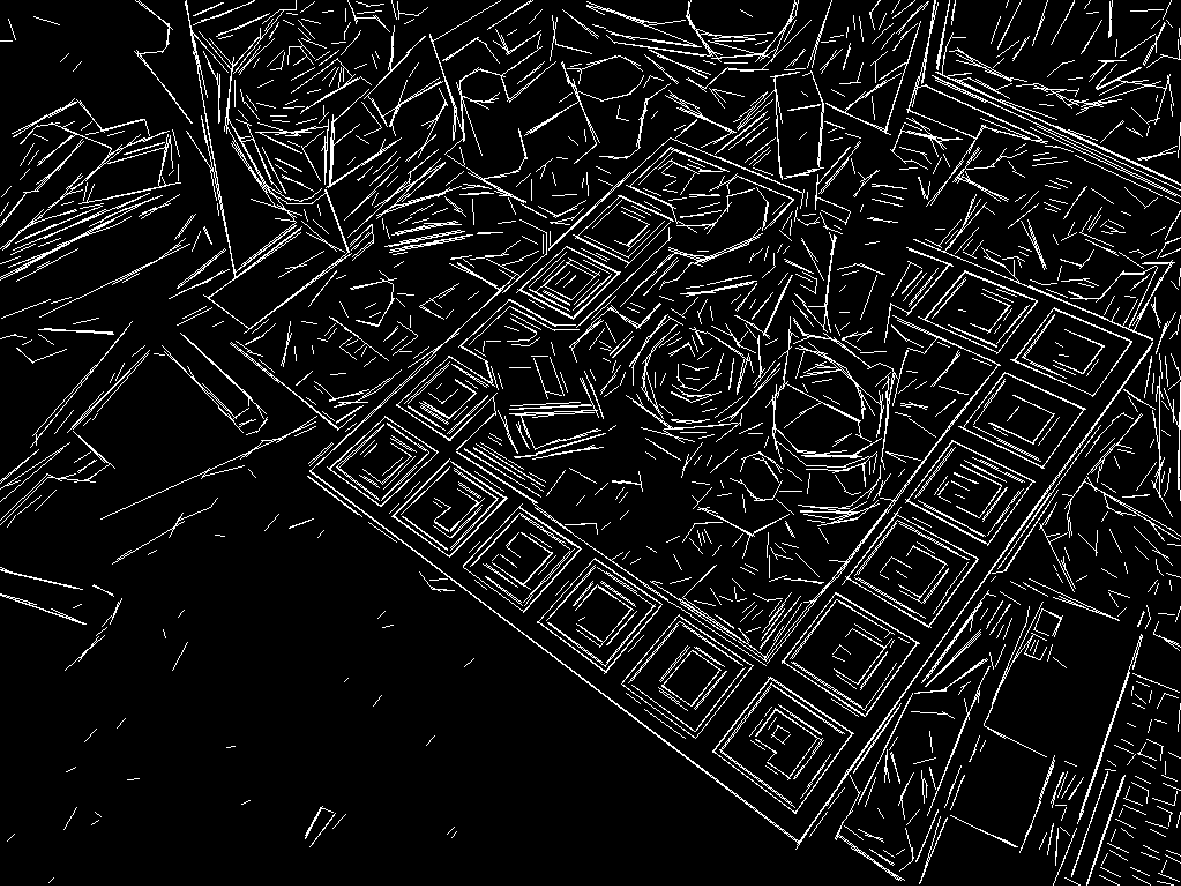
\includegraphics[height=3.5cm]{lsd}
    }
  \caption{边缘提取算法对比}
  \label{fig:chap03:edge_extra}
\end{figure}

完成边缘图像提取之后,需要根据该图像计算~DCM~张量。为加速~DCM~张量的方向误差计算,本文将按一定角度间隔~$\varepsilon$~对边缘方向进行离散化,使得各角度范围内的边缘单独成图。$\varepsilon$~的取值
将会对计算精度以及计算速度造成影响,$\varepsilon$~越小,细分方向范围也就越多,方向距离的精度也就越高,但计算量也随之提高。考虑精度要求以及算法时效性的辩证关系,通过测试选择$\varepsilon=3^\circ$,
即将边缘方向分为60个离散的方向范围,每个范围角度差为~$3^\circ$,如图~\ref{fig:chap03:direct_edge}~所示为使用图~\ref{fig:chap03:lsd}~进行边缘离散化之后的示意图,从左到右依次表示角度范围为:
$\theta=0^\circ\sim 3^\circ,~33^\circ\sim 36^\circ,~81^\circ\sim 84^\circ,~117^\circ\sim 120^\circ,~177^\circ\sim 180^\circ$~的离散边缘图。
之后对各方向范围的边缘图像计算二维倒角张量~(CM),即寻找图像中所有像素点距离当前边缘图像中最近边缘点的图像距离,并将该图像距离作为该像素点的灰度值。若当前像素点即为边缘点,则将其灰度值设为0。
因此距离图像边缘越近的像素点,其灰度值越小,图像显示越暗;距离图像边缘越远的像素点,其灰度值越大,图像显示越亮,如图~\ref{fig:chap03:CM_tensor}~所示,为相应离散角度范围的边缘图计算所得的~CM~张量
$DT_{V\{\hat{\phi}_i\}}$,其中$\hat{\phi}_i,~i=\{1,\dotsc ,60\}$代表离散边缘的方向,$V$代表当前场景图像。各角度的方向倒角距离~$DT3_{V\{\hat{\phi}_i\}}$将以$DT_{V\{\hat{\phi}_i\}}$作为初始值,使用双向
动态规划算法寻找各像素点的最小方向倒角距离,如式~(\ref{equ:chap03:dt3v})~为双向动态规划的计算公式,其中~$\lambda$~代表方向误差权重,$x$~代表图像中的任一像素点。
\begin{equation}
  \label{equ:chap03:dt3v}
  \left\{
    \begin{aligned}{}
      DT3_V(x,\hat{\phi}_i)=min\{DT3_V(x,\hat{\phi}_i), DT3_V(x,\hat{\phi}_{i-1})+\lambda\lVert \hat{\phi}_{i-1}-\hat{\phi}_{i}\rVert_\pi\}\\
      DT3_V(x,\hat{\phi}_i)=min\{DT3_V(x,\hat{\phi}_i), DT3_V(x,\hat{\phi}_{i+1})+\lambda\lVert \hat{\phi}_{i+1}-\hat{\phi}_{i}\rVert_\pi\}
    \end{aligned}
    \right.
\end{equation}

该方法计算速度快,在初始状态,将所有像素点的~$DT3_V$~设置为其倒角距离张量~$DT_V$,通过验证,该方法能够在最多~1.5~次前向与后向循环之后,得到各角度边缘图像中的所有像素点所对应的最小方向倒角距离\cite{LiuFastObjectLocalization2012}。计算
时间复杂度控制在~$O(q)$~以内,其中~$q$~代表图像的像素个数。如图~\ref{fig:chap03:DCM_tensor}~所示,为相应角度边缘图像计算所得的~DCM~张量。

\begin{figure}[t] %[h]
  \centering%
  \subcaptionbox{方向离散化边缘图\label{fig:chap03:direct_edge}}{%    
    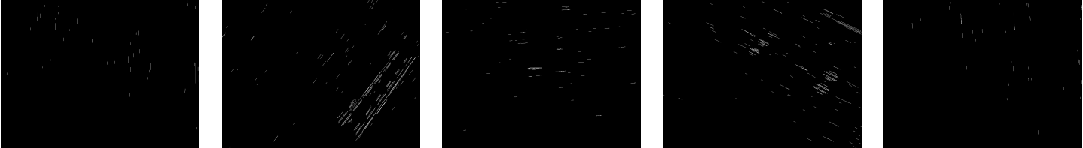
\includegraphics[height=2cm]{direct_edge}}\vskip0.2cm
  \subcaptionbox{CM~二维张量\label{fig:chap03:CM_tensor}}{%  
    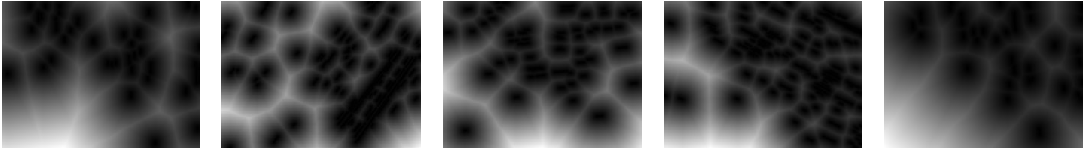
\includegraphics[height=2cm]{direct_cm}}\vskip0.2cm
  \subcaptionbox{DCM~三维张量\label{fig:chap03:DCM_tensor}}{%  
    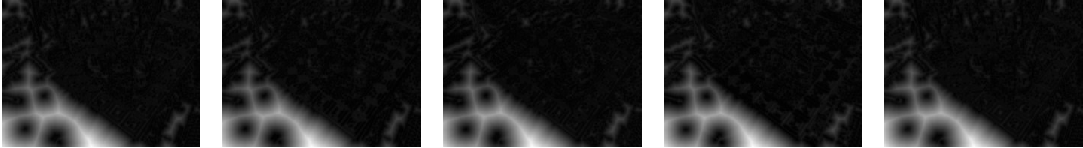
\includegraphics[height=2cm]{direct_dcm}}
  \caption{方向离散化张量示意图}
  \label{fig:chap03:direct_tensor}
\end{figure}

\subsection{模型投影以及目标函数构建} 
\label{sec:Objective function Building}
基于~DCM~构建目标函数需要确定物体模型边缘点在相机成像平面的图像坐标。即通过初始位姿与物体三维模型,根据相机投影模型计算物体边缘的图像坐标,以得到位姿优化的目标函数。

首先通过初始位姿确定物体三维模型相对于相机的位置,如图~\ref{fig:chap03:pose_init}~所示,在首帧图像中,该位姿由初始化算法得到,而在之后的追踪过程中,该位姿为上一帧得到的物体位姿。初始状态为粗匹配位姿,需要在此基础上通过优化算法得到目标物体在
相机坐标系中的精确位姿。

\begin{figure}[t] %[h]
  \centering%
  \subcaptionbox{初始位姿调整\label{fig:chap03:pose_init_camera}}{%    
  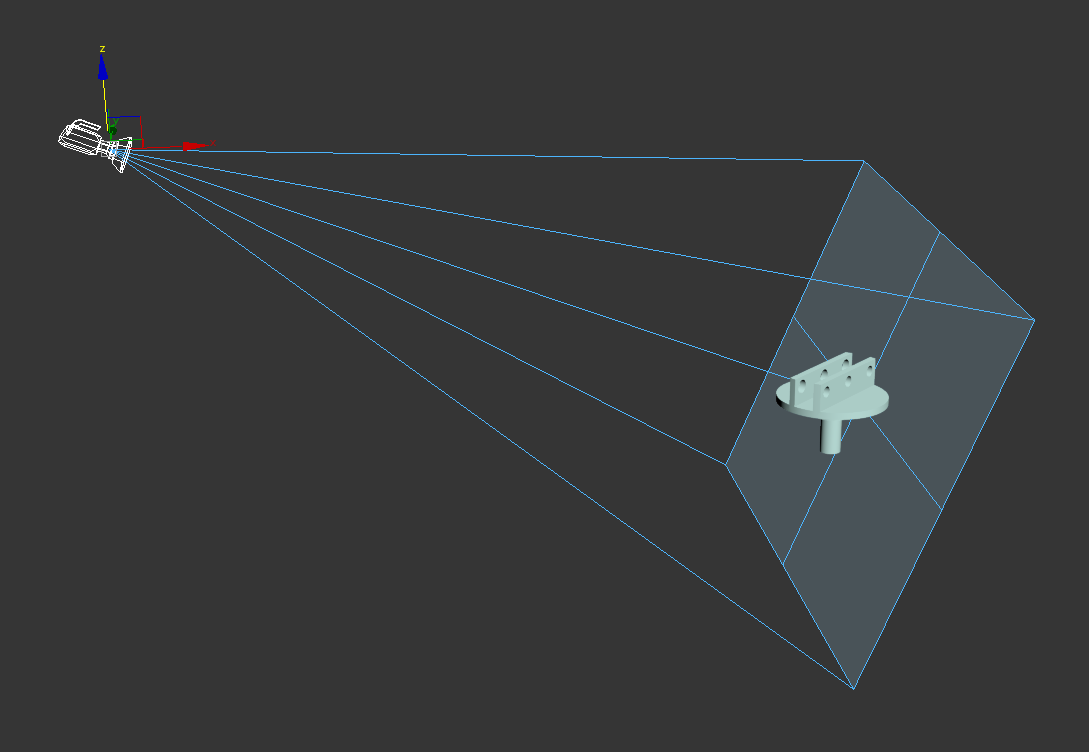
\includegraphics[height=5cm]{pose_init}}\hspace{1em}%\vskip0.2cm
\subcaptionbox{相机视野\label{fig:chap03:init_in_cam}}{%  
  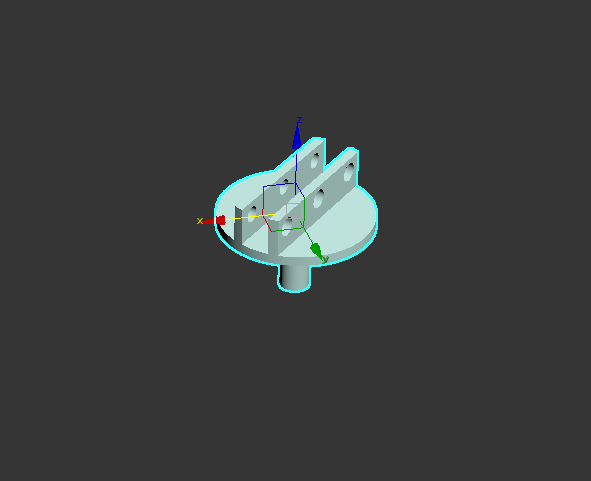
\includegraphics[height=5cm]{init_in_cam}}%\vskip0.2cm
  \caption{物体相对位姿初始化}
  \label{fig:chap03:pose_init}
\end{figure}

之后根据物体三维模型相对于相机的位姿关系,寻找物体边缘在场景图像中的投影。直接投影物体模型需要对边缘进行线段化,并且在出现较短或者曲向边缘时,计算将更为繁琐与复杂。因此本文采用
对三维模型边缘进行光栅化的方法。三维模型边缘点提取步骤为:(1)使用~OpenGL~的~Z-buffer~进行三维模型的边缘提取。在确定模型相对于相机的位姿后,可以通过投影方法计算场景中所有点在相机坐标系中的深度,之后通过寻找深度值变化的突变以提取模型的边缘直线,
如图~\ref{fig:chap03:model_edge_line}~所示。该方法能够仅提取当前位姿关系下的可见边缘,依靠对比投影到相同像素点的深度,仅保存距离最小的点的投影,以去除被遮挡边缘对最终结果的影响。(2)对所得模型边缘直线进行光栅化。在所得边缘直线上
等间距提取边缘点集~$P=\{o_1,\dotsc ,o_m\}\in\mathbb{R}^3 $,如图~\ref{fig:chap03:model_edge_guangshan}~所示。由于光栅点的个数影响后期目标函数的残差数量,进而影响算法的效率,因此需要权衡追踪精度与算法时效的关系,
本文选择光栅点间距在~$1\sim 2mm$。在物体模型尺寸较大时可以适当扩大该间距以减少过多的光栅点。(3)在边缘光栅点的边缘切向方向上继续提取光栅点集~$\overline P=\{\overline o_1,\dotsc ,\overline o_m\}\in\mathbb{R}^3 $,使得:
\begin{equation}
  \label{equ:chap3:dir_point}
\overline o_i=o_i+\hat \tau (o_i)\cdot dr
\end{equation}
其中~$\hat \tau (\cdot)$~代表边缘切向向量,$dr$~代表图像距离上的微小增量,$0<dr\ll 1$。$\overline P$~点集位于~$P$~点集的边缘切向方向上,两者的连线方向即代表相应的模型边缘方向。

最后使用初始位姿以及相机投影模型将点集映射到图像平面。假设初始位姿为~$g\in SE(3)$,代表位姿优化前物体相对于相机的旋转与平移关系,由式~(\ref{equ:chap3:localization})~将三维点集映射到图像坐标系,
其中~$x_i$~与~$\overline x_i$~分别代表~$o_i$~与~$\overline o_i$~在图像平面中的映射点,~$\pi (\cdot)$~代表相机投影模型。
\begin{equation}
  \label{equ:chap3:localization}
  \left\{
    \begin{aligned}{}
      x_i=\pi(o_i,g)\in \mathbb{R}^2,i=\{1,\dotsc ,m\}\\
      \overline x_i=\pi(\overline o_i,g)\in \mathbb{R}^2,i=\{1,\dotsc ,m\}
    \end{aligned}
    \right.
\end{equation}

\begin{figure}[t] %[h]
  \centering%
  \subcaptionbox{模型边缘提取\label{fig:chap03:model_edge_line}}{%    
    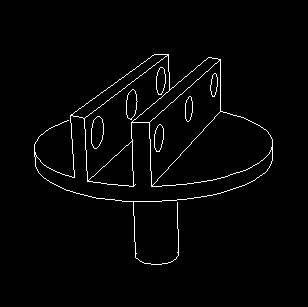
\includegraphics[height=4.5cm]{model_edge}}\hspace{0.5em}%\vskip0.2cm
  \subcaptionbox{边缘光栅化\label{fig:chap03:model_edge_guangshan}}{%  
    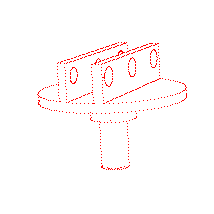
\includegraphics[height=4.5cm]{tmp7}}\hspace{0.5em}%\vskip0.2cm
  \subcaptionbox{初始位姿光栅点投影\label{fig:chap03:init_localization}}{%  
    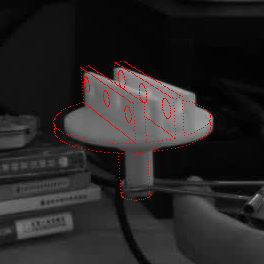
\includegraphics[height=4.5cm]{init_localization}}
  \caption{模型边缘提取与投影}
  \label{fig:chap03:model_edge_extra_local}
\end{figure}

由于点集$\overline P$是由点集$P$在三维模型边缘切向上增加微小距离得到的点集,因此投影后,二维点集~$x_i$~与~$\overline x_i$~的连线方向即为投影后的模型边缘方向,记为~$\phi (x_i)$,其中~$i=\{1,\dotsc ,n\}$,$n$~代表模型光栅点的数量。

完成模型边缘光栅点的提取、映射以及场景图像~DCM~张量计算后,通过光栅点的图像坐标~$x_i$~以及该模型边缘点的方向~$\phi (x_i)$~构造方向倒角匹配残差函数:
\begin{equation}
  \label{equ:chap3:dir_directional_function}
  E_{DCM}=\frac{1}{2}\sum _{i=1}^n DT3_V(x_i,\hat \phi(x_i))
\end{equation}
其中~$n$~代表模型边缘点的数量,$\hat \phi(x_i)$~为包含模型边缘方向的离散角度范围,。该离散范围是对场景边缘图像进行方向离散化的角度范围。
即通过模型边缘方向选择对应的离散场景边缘图像,在如图~\ref{fig:chap03:DCM_tensor}~所示的各角度~DCM~张量图中,寻找对应角度张量图。并边缘点的图像坐标~$x_i$~得到该点的~DCM~张量作为相应的优化函数残差。
最后通过叠加所有模型光栅点的~DCM~张量构造优化的残差函数。

通过构造后的残差函数作为优化的目标函数,将匹配问题转化为寻优问题,寻找使得所有边缘光栅点匹配残差之和最小的相对位姿。设物体相对于相机的旋转向量~$R=[r_x~r_y~r_z]^{\textrm{T}}$~以及平移向量
~$\textrm{T}=[t_x~t_y~t_z]^{\textrm{T}}$,由此根据残差函数得到优化的目标函数:
\begin{equation}
  \label{equ:chap3:dir_func}
  E_{DCM}=\frac{1}{2}\sum _{i=1}^n DT3_V[\pi (o_i,g(\textrm{T},R)),\hat \phi(\pi (o_i,g(\textrm{T},R)))]^2
\end{equation}
其中,$o_i$~代表三维模型边缘光栅点,$\pi(\cdot)$~代表相机投影模型,$g(\textrm{T},R)\in \mathbb{R}^6$~代表物体相对于相机的位姿,在优化初始阶段为给定的初始位姿。通过优化目标函数~$E(\textrm{T},R)$~以获得当前帧中物体相对于相机
的精确位姿变换关系,并将该帧位姿作为下一帧图像的初始位姿,以实现姿态追踪。
\section{追踪系统目标函数寻优}
\label{sec:Optimization of objective function}
位姿优化目标函数是关于场景~DCM~张量、相机投影模型、物体三维模型以及相对位姿的函数;在完成场景边缘提取以及相机标定后,目标函数中的自变量仅剩物体相对于相机的位姿。求解使得目标函数最小的相对位姿
即为物体模型与场景边缘图像的最优匹配,即为精确的相对位姿。本节将会讨论目标函数的寻优方法。
\subsection{数值导数寻优方法}
\label{sec:optimizing numerical derivative}
寻找目标函数相对于自变量的微分是寻优问题的关键,但对于复杂问题,计算其雅可比矩阵将会十分复杂或者无解析解,因此出现了有限差分方法。该方法通过在函数中给定无限小的摄动后,计算函数值的改变,如式~(\ref{equ:chap3:num_dir})~所示,以此
作为函数在该点处的数值导数。
\begin{equation}
  \label{equ:chap3:num_dir}
  \frac{\partial f}{\partial x_i}\approx \frac{f(x_i+\epsilon)-f(x_i-\epsilon)}{2\epsilon}
\end{equation}

目标函数的待优化变量为相对位姿变换~$g(\textrm{T},R)\in \mathbb{R}^6$~,其中包括物体相对相机坐标系的旋转向量~$R=[r_x~r_y~r_z]^\textrm{T}$~以及平移向量~$\textrm{T}=[t_x~t_y~t_z]^\textrm{T}$。
该函数十分复杂,难点在于~DCM~张量是通过场景边缘图像计算而来,并且对边缘图像进行了方向离散化与双向动态规划,该过程无法直接建模,并且计算过程耦合了相机投影模型,进一步提高了雅可比矩阵的计算难度。
因此~Imperoli~等人~\cite{ImperoliD2COFastRobust2015}使用数值偏导方法对目标函数进行寻优。

该方法通过寻找位姿摄动~$\Delta g$,使目标函数不断接近最小值。最终在迭代一定次数或目标函数在前后迭代中的改变量低于一定阈值后停止,并得到最终的相对位姿。
迭代寻优的关键是寻找位姿摄动量,在给定优化步长的情况下,需要寻找使得目标函数下降最快的~$\Delta g$。由于位姿变换关系~$g(\textrm{T},R)$~含有六个变量,计算时将分别对六个单独的位姿量加入摄动,在其他五个位姿
关系不变的情况下,寻找使得目标函数下降最快的改变量作为当前变量的摄动。寻找到六个变量的最优摄动后,将它们组合作为该步的位姿改变量,并将其叠加到初始位姿,以获得该步迭代的位姿结果。设~$M$~代表场景的
灰度图像,$m$~代表目标物体的三维模型,$g_{ini}$~代表优化前的初始位姿,$step$~代表迭代过程中的最大步长。采用数值偏导求导位姿的流程如算法~\ref{alg:num_dir}~所示。
\begin{algorithm}[H]
  \caption{[$g$]=Num-deri($M$,$m$,$g_{ini}$,$step$)}
  \label{alg:num_dir}
  \begin{algorithmic}[1]
    \Require{$M$,$m$,$g_{ini}$,$step$}
    \State 提取场景边缘图像。
    \State 根据~(\ref{equ:chap03:dt3v})~计算~$DT3_V$.
    \State 根据~(\ref{equ:chap3:localization})~计算投影光栅点。
    \State 构建位姿优化目标函数~$E_{DCM}$.
    \State 令~$g=g_{ini}$~.
    \Repeat
    \State 寻找使得~$DT3_V$~下降最快的~$\Delta g$.
    \Statex \hspace{0.2cm} $\Diamond$ 单次迭代的~$\Delta g$~步长需控制在~$step$~以内。
    \State 叠加~$\Delta g$~至~$g$~得到该次迭代位姿优化结果。
    \State 通过~(\ref{equ:chap3:localization})~更新投影点位置。
    \State 通过~(\ref{equ:chap3:dir_func})~更新优化目标函数。
    \Until{达到最大迭代次数,或者相邻迭代中目标函数的改变足够小。}
    \\
    \Return {$g$}
  \end{algorithmic}
\end{algorithm}

使用数值导数寻优的方法在选取合适步长以及背景较为简单的情况下能够取得不错的效果。但出现噪音较大、背景过于复杂的情况容易出现边缘误匹配。当在物体边缘附近出现与其平行的背景边缘时,算法容易陷入局部最小值,
将模型边缘匹配到背景边缘。为解决该问题,本文将提出解析偏导寻优方法,通过寻找相对位姿与光栅点的解析偏导,提高寻优精度。

\subsection{解析偏导矩阵计算}
\label{sec:Matrix calculation}
为提高位姿配准的精度,提高算法鲁棒性,避免优化过程陷入局部最小值,本文在原有算法基础上提出改进的寻优方法。
分析目标函数~$E(\textrm{T},R)$,其是由场景~$DT3_V$~张量、模型映射到图像中的二维图像坐标点集~$x_i(u_i,v_i)$~以及该点集的边缘方向~$\hat \phi (x_i)$~确定,而待优化变量为目标物体相对于相机的位姿
变换~$g(\textrm{T},R)$。由于边缘图像无法解析化并且双向动态规划算法也无解析解,导致直接寻找目标函数相对于待优化变量的偏导十分困难。当场景边缘图像以及相机模型确定后,目标函数中仅有映射点坐标为自变量。
因此本文尝试使用位姿变换关系~$g(\textrm{T},R)$~相对于图像映射点坐标~$x_i(u_i,v_i)$~的雅可比矩阵,解析地表示相对位姿的变化对物体映射点的坐标的变化关系,之后通过所计算的二维图像坐标变换求解
相应光栅点的~$DT3_V$~改变,以计算位姿变换对目标函数的改变,以得到待优化变量的偏导。

假设目标物体坐标系为~$C_{obj}$,相机坐标系~$C_{cam}$~,$C_{obj}$~相对于~$C_{cam}$~的一次变换为~$G$~(对应李代数为~$\xi$,对应旋转矩阵~$R$~以及平移向量~$\mathbf{t}$),现存在目标物体坐标系~$C_{obj}$~上一点
~$p$,其位于~$C_{cam}$~中的位置为~$Gp$。给定~$G$~左乘一个扰动~$\Delta G=\textrm{exp}(\delta \xi^\wedge)$,$~^\wedge$~算符代表求取向量的反对称矩阵,并设定扰动项的李代数为~$\delta \xi =[\delta \rho , \delta \phi]^{\textrm{T}}$,可得\footnote{详细推导过程见:高翔,张涛编著:《视觉~SLAM~十四讲》,北京:电子工业出版社2017年版,第72-76页。}:
\begin{align}
    \label{equ:chap3:lidaishu}
    \begin{split}
  \frac{\partial (Gp)}{\partial \delta \xi}&=\lim_{\partial \xi \to 0}\frac{\textrm{exp}(\delta \xi ^\wedge)\textrm{exp}(\xi^\wedge)p-\textrm{exp}(\xi^\wedge)p}{\delta \xi} \\
                                          &\approx \lim_{\partial \xi \to 0}\frac{(\textrm I+\delta \xi ^\wedge)\textrm{exp}(\xi^\wedge)p-\textrm{exp}(\xi^\wedge)p}{\delta \xi} \\
                                          &=\lim_{\partial \xi \to 0}\frac{\delta \xi^\wedge\textrm{exp}(\xi ^\wedge)p}{\delta \xi}=\lim_{\partial \xi \to 0}\frac{\left( \begin{matrix}\partial\phi^\wedge (Rp+\mathbf{t})+\delta p\\
                                                                                                                                                                            0 \end{matrix}\right)}{\partial \xi} \\
                                          &=\left[ \begin{matrix}  
                                          \textrm{I} & -(Rp+\mathbf{t})^\wedge\\
                                          \mathbf{0}^{\textrm{T}} & \mathbf{0}^{\textrm{T}}
                                          \end{matrix}\right]
    \end{split}
\end{align}
记点~$p$~变换到相机坐标系后的点为~$p'=[x',y',z']^T$,~$p'$~映射到相机图像平面的对应点为~$e=[u,v]$~,式~(\ref{equ:chap3:lidaishu})~转换为:
\begin{equation}
  \label{equ:chap3:lidaishu_deri}
\frac{\partial (p')}{\partial \delta \xi}=\left[ \begin{matrix} \textrm{I} & -(Rp+\mathbf{t})^\wedge \\ \mathbf{0}^{\textrm{T}} & \mathbf{0}^{\textrm{T}}  \end{matrix}\right]
\end{equation}
根据相机投影模型,其中~$f_x,f_y,c_x,c_y$~分别代表相机在~x~轴和~y~轴的焦距以及光心坐标,对于点~$p'$:
\begin{equation}
  \label{equ:chap3:point_proj}
\left[\begin{matrix} su  \\ sv\\ s \end{matrix}\right]=\left[ \begin{matrix} f_x & 0 & c_x \\ 0 & f_y & c_y \\ 0 & 0 & 1\end{matrix}\right]\left[ \begin{matrix} x' \\ y' \\z' \end{matrix}\right]
\end{equation}
使用第三行消去点~$p'$~距离相机坐标系的距离~$s$,使得:
\begin{equation}
  \label{equ:chap3:u_and_v}
  \left\{
    \begin{aligned}{}
      u=f_x\frac{x'}{z'}+c_x \\
      v=f_y\frac{y'}{z'}+c_y
    \end{aligned}
  \right.
\end{equation}
由此计算偏导数可得:
\begin{equation}
\label{equ:chap3:partial_of_loc}
\frac{\partial e}{\partial (p')}=-\left[ \begin{matrix}   
  \frac{\partial u}{\partial x'} & \frac{\partial u}{\partial y'} &  \frac{\partial u}{\partial z'} \\
  \frac{\partial v}{\partial x'} & \frac{\partial v}{\partial y'}  & \frac{\partial v}{\partial z'}
\end{matrix}\right]=-\left[
\begin{matrix}
  \frac{f_x}{z'} & 0 &  -\frac{f_xx'}{z'^2} \\
  0 & \frac{f_y}{z'}  & -\frac{f_yy'}{z'^2}
\end{matrix}  
\right]
\end{equation}
根据式~(\ref{equ:chap3:lidaishu_deri})~以及~(\ref{equ:chap3:partial_of_loc})~可得物体上一点投影到图像平面内得坐标相对于坐标系变换关系得雅可比矩阵:
\begin{equation}
  \label{equ:chap3:yakebi}
\frac{\partial e}{\partial \delta \xi}=-\left[ \begin{matrix}   
\frac{f_x}{z'} & 0 & -\frac{f_xx'}{z'^2} & -\frac{f_xx'y'}{z'^2} & f_x+\frac{f_xx'^2}{z'^2} & -\frac{f_xy'}{z'} \\
0 & \frac{f_y}{z'} & -\frac{f_yy'}{z'^2} & -f_y-\frac{f_yy'^2}{z'^2} & \frac{f_yx'y'}{z'^2} & \frac{f_yx'}{z'}
\end{matrix} \right]
\end{equation}

该雅可比矩阵代表了相对位姿摄动~$\delta \xi$~与物体上一点在图像平面的投影坐标的微分关系,即~$\frac{\partial e}{\partial \delta \xi}=\frac{\partial e(u_i,v_i)}{\partial g(t_x,t_y,t_z,r_x,r_y,r_z)}$,其中~$u_i,v_i$~分别代表
投影点在图像平面中的横纵坐标,$t_x,t_y,t_z,r_x,r_y,r_z$~代表目标物体相对于相机的位姿关系。
\subsection{解析导数寻优方法}
\label{sec:Analytic derivative optimization}
物体边缘投影点坐标直接确定了位姿优化的目标函数,因此解析求解位姿变化相对于投影点坐标的偏导将提高位姿匹配的精度。
通过给定相对位姿一定的摄动,首先根据式~(\ref{equ:chap3:yakebi})~计算投影点坐标的相对改变,再通过坐标的改变计算位姿优化的残差,且计算最速下降~$\Delta e$~的过程将比计算最速下降~$\Delta g$~简单,通过在对应
~$DCM$~张量中寻找一定步长内的最小值作为该光栅点的优化残差,使用非线性最小二乘法对目标函数进行寻优\footnote{本文使用~Google Ceres-Solver~对目标函数进行寻优:http://ceres-solver.org/},以得到优化位姿,改进后的方法如算法~\ref{alg:Analytical}~所示。
\begin{algorithm}[H]
  \caption{[$g$]=Analy-deri($M$,$m$,$g_{ini}$,$step$)}
  \label{alg:Analytical}
  \begin{algorithmic}[1]
    \Require{$M$,$m$,$g_{ini}$,$step$}
    \State 提取场景边缘图像。
    \State 根据~(\ref{equ:chap03:dt3v})~计算~$DT3_V$.
    \State 根据~(\ref{equ:chap3:localization})~计算投影光栅点。
    \State 构建位姿优化目标函数~$E_{DCM}$.
    \State 令~$g=g_{ini}$~.
    \Repeat
    \State 寻找使得~$DT3_V$~下降最快的~$\Delta e$.
    \Statex \hspace{0.5cm} $\Diamond$ 单次迭代的~$\Delta e$~步长需控制在~$step$~以内。
    \State 根据~(\ref{equ:chap3:yakebi})~求解~$\Delta g$.
    \State 叠加~$\Delta g$~至~$g$~得到该次迭代位姿优化结果。
    \State 通过~(\ref{equ:chap3:localization})~更新投影点位置。
    \State 通过~(\ref{equ:chap3:dir_func})~更新优化目标函数。
    \Until{达到最大迭代次数,或者相邻迭代中目标函数的改变足够小。}
    \\
    \Return {$g$}
  \end{algorithmic}
\end{algorithm}
\vspace{6pt} 

利用解析偏导替代数值偏导的方法能够提高寻优结果的精度,如图~\ref{fig:chap03:compare_Optimiz}~为两种寻优方法的效果对比图,其中图~\ref{fig:chap03:compare_init_pose}~为优化
前的初始位姿,图~\ref{fig:chap03:compare_shuzhi_deri}~为使用数值偏导寻优的结果,物体的部分边缘出现了误匹配,其原因是优化过程陷入了局部最小值,模型的部分边缘匹配准确,但也存在一定边缘由于背景影响
出现了误匹配,甚至某些边缘完全无法匹配至图像边缘。
图~\ref{fig:chap03:compare_jiexi_deri}~为使用解析偏导进行寻优的结果,相比数值偏导,物体模型的所有边缘皆匹配至正确的场景边缘,物体三维模型与场景边缘图像的配准良好,相对位姿的计算也将更加精准。

\begin{figure}[t] %[h]
  \centering%
  \subcaptionbox{初始给定位姿\label{fig:chap03:compare_init_pose}}{%    
    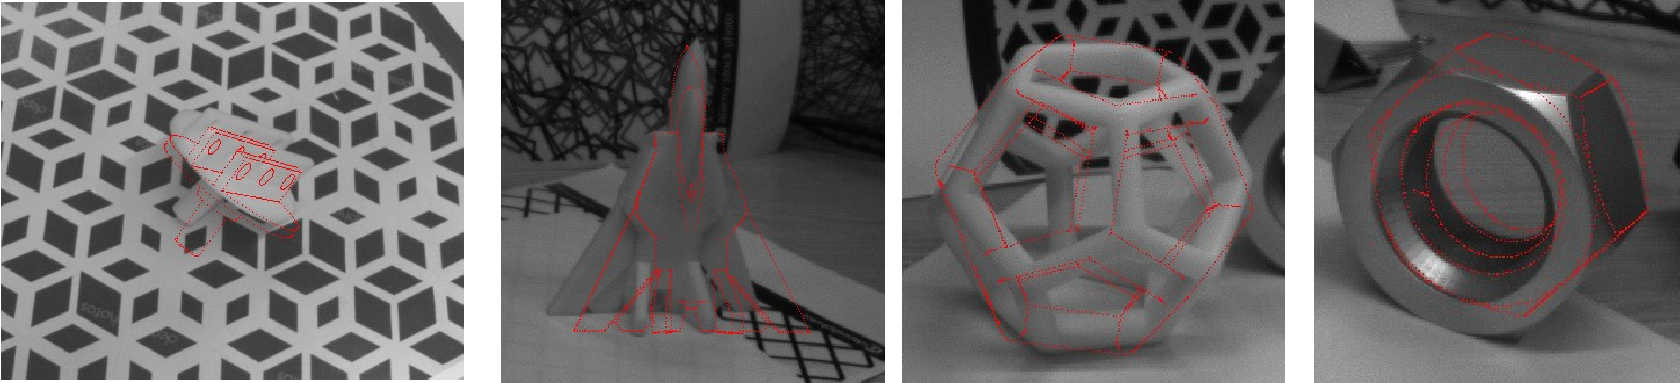
\includegraphics[height=3cm]{compare_init_pose}}\vskip0.2cm
  \subcaptionbox{数值偏导优化结果\label{fig:chap03:compare_shuzhi_deri}}{%  
    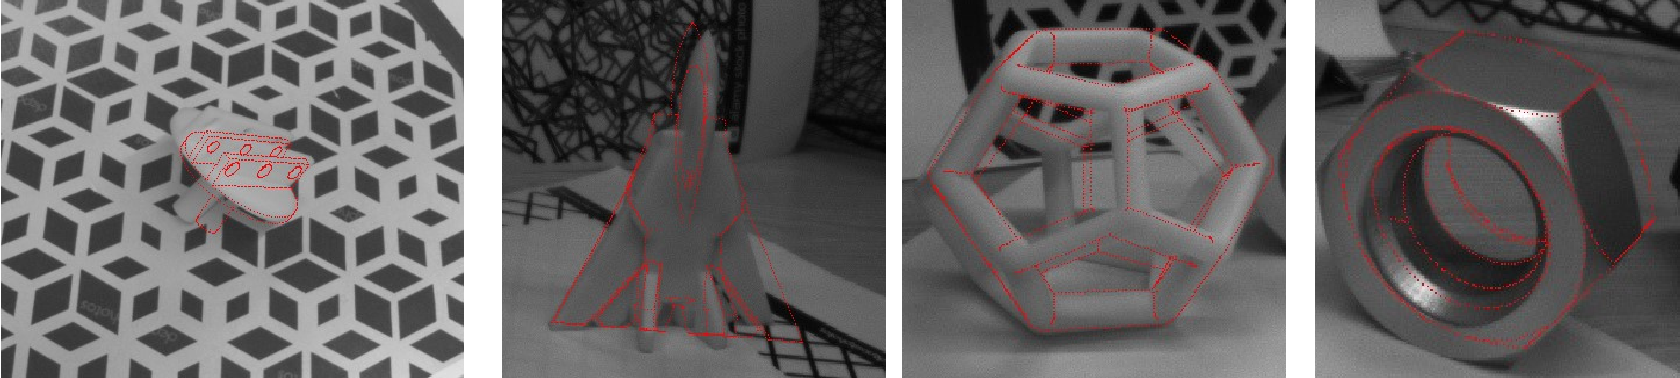
\includegraphics[height=3cm]{compare_shuzhi_deri}}\vskip0.2cm
  \subcaptionbox{解析偏导优化结果\label{fig:chap03:compare_jiexi_deri}}{%  
    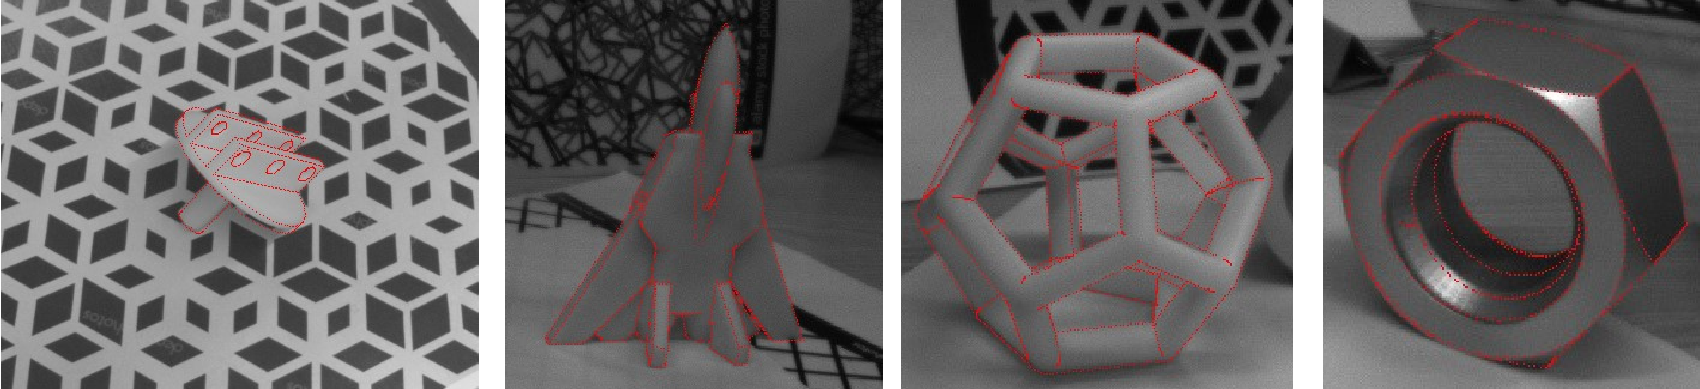
\includegraphics[height=3.1cm]{compare_jiexi_deri}}
  \caption{寻优方法对比图}
  \label{fig:chap03:compare_Optimiz}
\end{figure}

\section{自适应权重优化算法}
\label{sec:Weight optimization algorithm}
解析优化方法能够对贫纹理物体实现位姿追踪,且算法在背景较为复杂的情况下也能够实现稳定、准确的目标定位以及姿态跟随。但追踪算法常会由于遮挡等情况出现较大误差,因此本文针对该问题提出自适应权重优化算法,使用梯度
评价算法对物体三维模型边缘光栅点进行权重计算,使用各光栅点的优化权重改变位姿优化函数,使优化算法对物体被遮挡部分的权重下降,提高未被遮挡部分对整体优化的权重,使得算法对遮挡情况的鲁棒性更高。
\subsection{遮挡问题分析}
\label{sec:Analysis of occlusion problem}
追踪算法常使用物体模型或特征点对物体实现位姿追踪,但当目标物体被部分遮挡时,其特征将会部分丢失。若使用恒定模型对目标物体进行追踪,算法将易于在被遮挡部分进行错误匹配。
针对本文所提出的追踪算法,当出现遮挡后,物体部分边缘在图像中消失,但算法无法判别被遮挡的区域,进而在错误的场景边缘中寻找最优匹配,导致整体匹配出现较大误差。如图~\ref{fig:chap03:zhedang}~所示为
两个贫纹理目标互相遮挡的示意图,由图可知,在发生遮挡时,模型光栅点不应在原位置进行边缘匹配,若仍然寻找最优的~DCM~张量匹配将引入较大误差。
为解决遮挡问题,本文提出自适应权重优化算法,使被遮挡
部分对整体优化的权值降低,提高算法对复杂背景以及遮挡情况下的追踪精度以及鲁棒性。

\begin{figure}[t] %[h]
  \centering%
  %\subcaptionbox{\label{fig:chap03:zhedang1}}{%    
    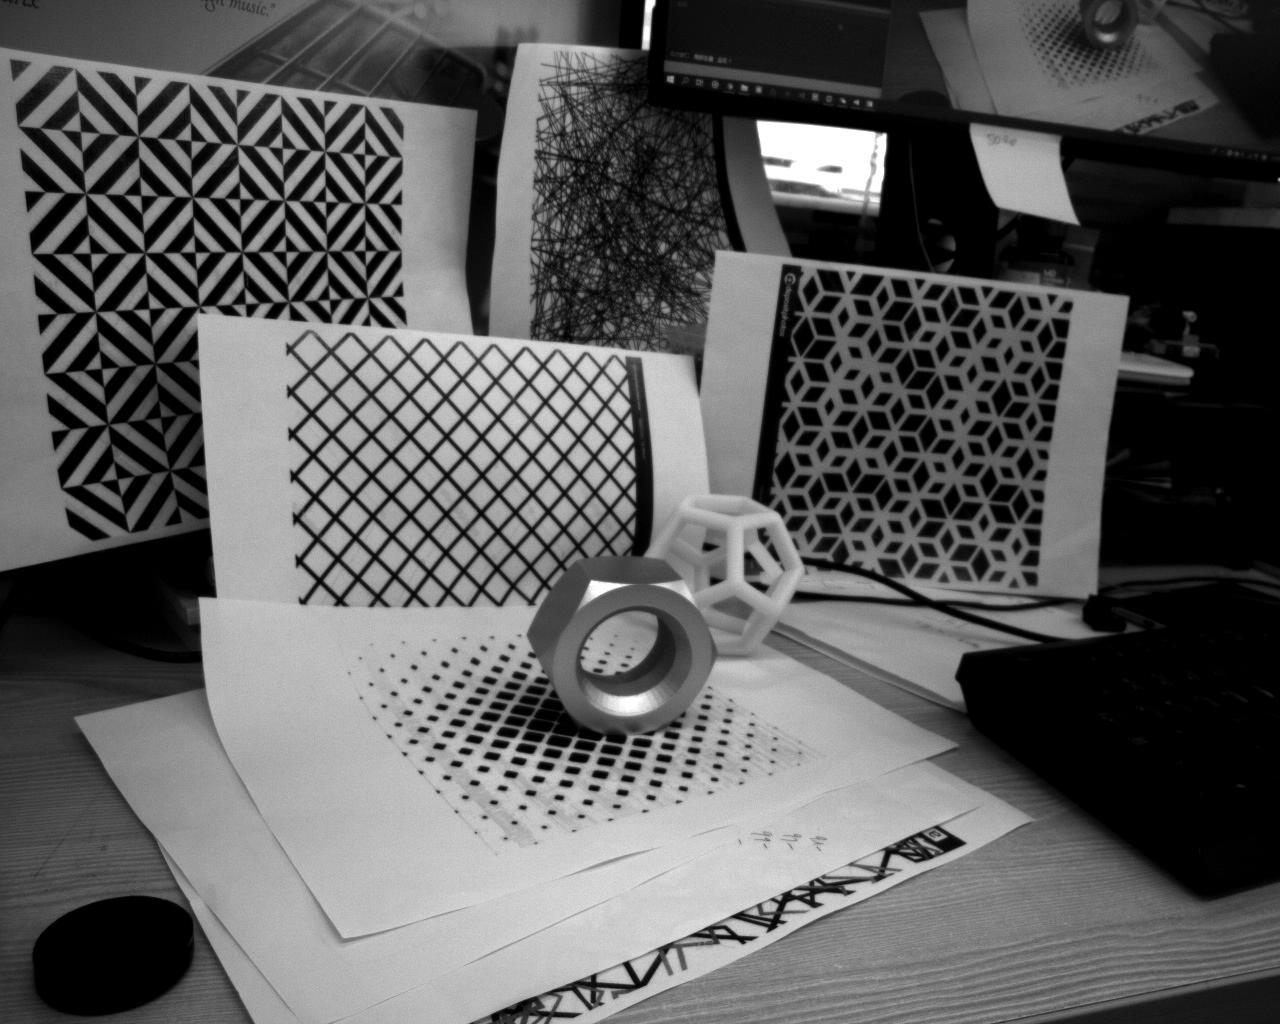
\includegraphics[height=5.3cm]{zhedang1}\hspace{2em}%\vskip0.2cm
  %\subcaptionbox{\label{fig:chap03:zhedang2}}{%  
    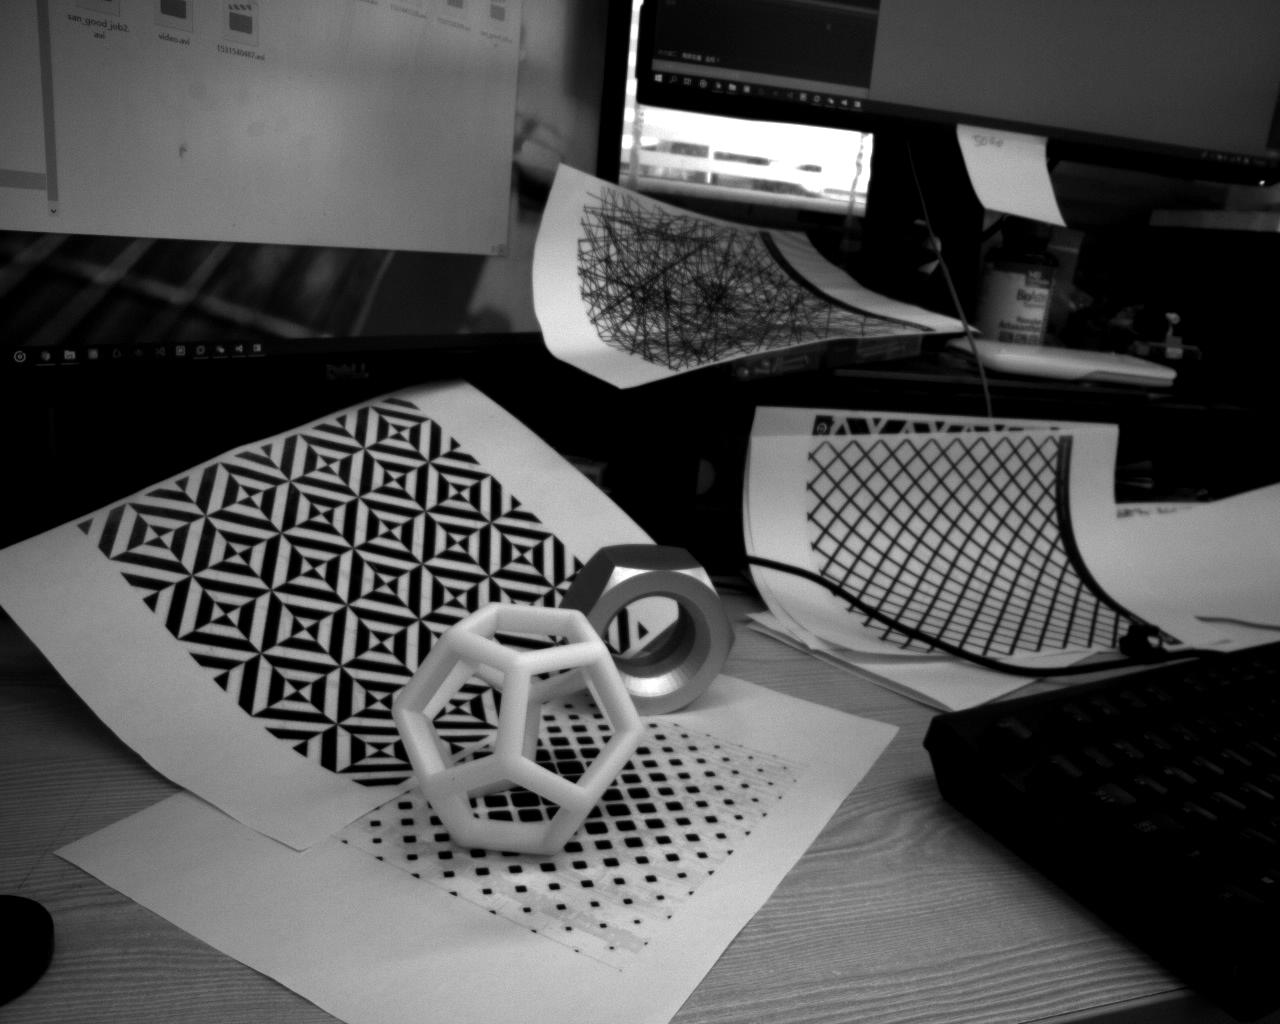
\includegraphics[height=5.3cm]{zhedang2}%\vskip0.2cm
  \caption{遮挡情况示意图}
  \label{fig:chap03:zhedang}
\end{figure}

\subsection{光栅点权重计算}
\label{sec:Direction weight Calculation}
本文将使用模型边缘点的方向以及所在图像位置的梯度以计算该点的优化权值,降低被遮挡点在目标函数中的权重,以使被遮挡点对整体寻优的干扰降低。在完成当前帧边缘图像与物体三维模型匹配寻优后,
获得了当前时刻物体相对于相机的精确位姿变换关系~$g(\textrm{T},R)$,通过该位姿变换关系能够将模型边缘光栅点集~$P=\{o_1,\dotsc ,o_m\}\in \mathbb{R}^3$~及用于求取模型边缘方向的点集~$\overline P=\{\overline o_1,\dotsc ,\overline o_m\}\in \mathbb{R}^3$~
映射为图像坐标系中的二维模型边缘点,即通过式~(\ref{equ:chap3:localization})~得到点集~$x$~以及~$\overline x$,由此通过两个点集的连线方向得到模型边缘点在图像中的边缘方向~$\phi(x_i)$。

在完成模型边缘方向计算后,再对场景图像的梯度进行提取。本文使用~Sobel~算子对梯度进行提取,该算子将梯度矩阵与图像矩阵做平面卷积,如式~(\ref{equ:chap3:sobel})~所示,计算图像灰度的梯度近似值。该算子所需运算资源
相对较少,并且其计算范围包含被计算点周围的~8~个临近点,能够降低噪音对梯度计算的影响。
\begin{equation}
  \label{equ:chap3:sobel}
    M_x=\left[
      \begin{matrix}
        +1&0&-1\\
        +2&0&-2\\
        +1&0&-1
      \end{matrix}\right]*A~~~
    M_y=\left[
      \begin{matrix}
        +1&0&-1\\
        +2&0&-2\\
        +1&0&-1
      \end{matrix}\right]*A
\end{equation}
式中~$A$~表示原始图像矩阵中以计算点为中心的~$3 * 3$~图像矩阵,由此计算图像中所有像素点的梯度大小:~$M=\sqrt{M_x^2+M_Y^2}$~,以及方向:~$D = \arctan (M_y / M_x)$。

模型边缘点优化权重的计算方法为:首先根据模型光栅点的图像坐标计算相应图像点处的梯度大小~$M_g(x_i)$~以及方向~$D_g(x_i)$;之后对所有光栅点处的梯度大小进行筛选,若对应点所在的图像梯度过小,证明该点
所处图像位置边缘信息不明显。导致该问题的原因有:(1)~该处边缘由于光照过暗或过曝而导致无法边缘不可见;(2)~该处边缘被遮挡;(3)~图像噪音导致边缘模糊。在上述情况中,使用该点残差带入位姿优化的目标函数都将引入较大误差,
因此应降低该类边缘点对下一帧位姿优化的权重,防止误匹配点对物体位姿追踪的影响;最后,若梯度大小大于阈值,则证明该匹配点已匹配至场景的图像边缘,但匹配的正确与否无法判断。因此本文使用图像的梯度方向与模型
边缘在图像中的投影方向以判断是否匹配成功,通过计算两者的正弦值作为该光栅点的优化权重,其夹角越接近~$90^\circ$,则说明物体边缘方向与场景图像的边缘方向越接近,正弦结果越接近~1,权重也就越大;若两者夹角
越接近~$0^\circ$,物体边缘方向与场景图像的边缘方向偏差也就越大,正弦结果越接近~0,权重越小。总结可得光栅点的优化权重计算方法如式~(\ref{equ:chap3:point_quanzhong})~所示。
\begin{equation}
  \label{equ:chap3:point_quanzhong}
  \Xi (x_i)=
  \left\{
    \begin{aligned}{}
    M_g(x_i)&,&M_g(x_i) < 0.01 \\
    \sin (\phi(x_i)-D_g(x_i))&,&M_g(x_i) \geq 0.01
    \end{aligned}
    \right.
\end{equation}
将光栅点的优化权重作为残差权重加入目标优化函数,如式~(\ref{equ:chap3:eval_obj_func})。权重高的光栅点优化残差高,反之,权重低的光栅点优化残差低,该算法使得寻优过程将优先降低权重高的光栅点的残差,而
对匹配到被遮挡或边缘提取不良好的图像边缘的光栅点优化降低。
也即使得配准过程能够偏重于配准良好的图像区域,而降低遮挡等情况引入的干扰。
\begin{equation}
\label{equ:chap3:eval_obj_func}
E_{eva}(\textrm{T},R)=\frac{1}{2}\sum_{i=1}^n \Xi(x_i)\cdot E_{DCM}(\textrm{T},R)
\end{equation}
将图像坐标点~$x_i$~转换为三维空间点~$o_i$~得到带权重的目标优化函数:
\begin{equation}
  \label{equ:chap3:eval_obj_func_oi}
  E_{eva}(\textrm{T},R)=\frac{1}{2}\sum_{i=1}^n \Xi(\pi (o_i,g(\textrm{T},R)))\cdot E_{DCM}(\textrm{T},R)
  \end{equation}
\subsection{权重优化算法}
\label{sec:Weight optimization algorithm2}
在对目标物体实现位姿追踪时,常会由于背景干扰以及遮挡情况而出现错误匹配,导致算法失效。针对前述边缘匹配追踪算法,本文提出带权重的位姿优化算法,将上节计算的光栅点权重用于位姿优化的目标函数,使位姿优化
更加趋向于配准效果良好的光栅点,并且降低误匹配点的权重。本文在每帧图片寻优完成后,计算光栅点处的图像梯度,以得到每个点对应的优化权值。如图~\ref{fig:chap03:quanzhong}~所示,使用不同颜色以区分各光栅点的权重值,
绿色点代表权重大于~0.8~的光栅点,红色点代表
权重低于~0.3~的光栅点,蓝色点代表权重在~0.3~至0.8之间的点。由图可知,算法在目标物体被部分遮挡时也能有效配准可见部分,并且得到准确的位姿。且目标物体在被遮挡部分的光栅点颜色多为红色以及蓝色,
证明本文所提算法能够较为准确的判断物体被遮挡部分,并且对图像噪音造成的边缘提取不准确的情况也有极大的抑制作用。

\begin{figure}[t] %[h]
  \centering%  
    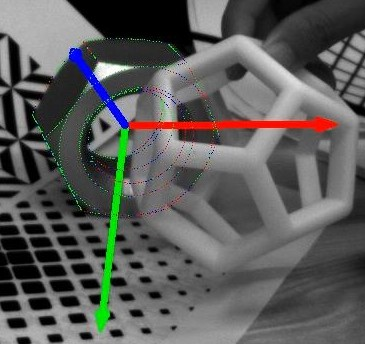
\includegraphics[height=6cm]{quanzhong2}\hspace{2em}%\vskip0.2cm
    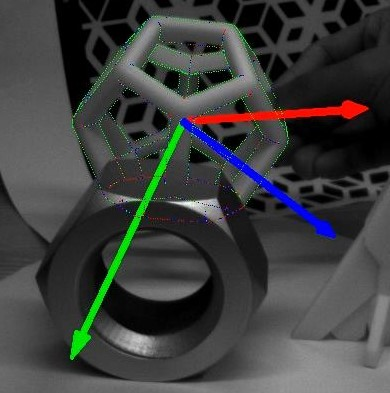
\includegraphics[height=6cm]{quanzhong3}%\vskip0.2cm
  \caption{自适应权重优化算法效果图}
  \label{fig:chap03:quanzhong}
\end{figure}

优化权重是由光栅点方向以及图像梯度方向的夹角计算所得,由于图像的梯度方向存在一定的偶然性,易于受到图像噪音以及背景边缘的干扰。例如在被遮挡部分出现了与光栅点方向垂直的图像边缘点,算法将错误地提高该点的权重,导致引入偶然误差。为解决该问题,
本文在完成光栅点的权值计算后,再对其进行中值滤波,使用距离光栅点一定范围内的临近光栅点的权重均值作为该点的权重,以降低突变权值点对整体寻优的影响。如代码~\ref{code:chap3:lvbo}~所示,首先通过模型的总光
栅点数确定单次滤波的光栅点数量~point\_num,该值下限为~10,以避免模型过小时,光栅点数量太少,导致中值滤波算法失效。之后在原始权重~pre\_weight~中,使用前后指针的方法在遍历一轮光栅点后计算出所有点的新权重~weight。该方法计算速度快,仅需遍历一次光栅点集的原始权重即可计算出通过中值
滤波后的权重。对权重进行中值滤波能够有效降低图像噪音以及背景边缘对优化权值的影响,提高光栅点权重的连续性。

%%\ttfamily,framexleftmargin=5mm,stepnumber=1,  numbersep=1pt, 

\begin{lstlisting}[
  language=C++,
  numbers=left,                
  numberstyle=\footnotesize,
  frame=single,     
  basicstyle=\small\tt,    
  caption={优化权重中值滤波的~C++~实现},
  label={code:chap3:lvbo}]
    int point_num = std::max(int(raster_pts.size()/100), 10);
    float sum_weight = 0;
    auto behind = pre_weight.begin();         
    auto front = pre_weight.begin() + point_num - 1;  
    std::vector<float>weight(pre_weight.size(), 0);                 
    for(int i = 0; i < point_num; i++)
    sum_weight += pre_weight[i];
    auto end_point = weight.begin() + point_num / 2;
    auto now = end_point;
    *now = sum_weight / point_num;
    now++;
    while (now != end_point) {
      front = \ 
      front + 1 == pre_weight.end() ? pre_weight.begin():++front;
      sum_weight += *front;
      sum_weight -= *front;
      behind++;
      *now = sum_weight / point_num;
      now = (now + 1 == weight.end()) ? weight.begin() : ++now;
    }
  \end{lstlisting}


\section{本章小结}
\label{sec:chapter3_summary}
本章通过模型与图像边缘匹配的方法,对贫纹理目标实现位姿追踪。该算法通过对图像边缘的提取以及三维模型的边缘提取和映射,
构建光栅点的方向倒角残差,利用匹配残差构造位姿优化的目标函数,之后通过目标函数的寻优实现物体的位姿追踪。该方法使用物体的三维模型进行追踪,相比特征点追踪方法,适用性更广。

然后针对目标函数的寻优方法进行改进。由于目标函数较为复杂,并且双向动态规划无解析的表达式,因此对目标函数的寻优常使用的是数值偏导方法。数值偏导寻优存在较大的误差,在背景较为复杂时,寻优将陷入局部最小值,
导致匹配失败。针对这一问题,本文通过寻找位姿变换与边缘映射点坐标的雅可比矩阵,改进寻优过程,提高配准精度,使算法在背景复杂的情况下也能精确追踪目标物体位姿。

最后重点研究了追踪过程中的遮挡问题,为解决该问题,本文提出了自适应权重优化算法。通过模型边缘方向与图像梯度方向以计算光栅点的优化权重,通过权重以降低被遮挡点的优化残差,
使匹配算法优先配准于未被遮挡的物体边缘。最后算法还对光栅点权重进行中值滤波,降低图像噪音以及背景误匹配导致的偶然误差。该算法能够及时有效地降低遮挡情况导致的边缘误匹配,提高目标追踪的精度以及鲁棒性。